\documentclass{ieeeaccess}

% IEEE Access template-based draft. Replace all AUTHOR_* placeholders before submission.
\usepackage{cite}
\usepackage{amsmath,amssymb,amsfonts}
\usepackage{algorithmic}
\usepackage{graphicx}
\usepackage{textcomp}
\usepackage{booktabs}
\usepackage{tabularx}
\usepackage{array}
\usepackage{url}
\usepackage{bm}
\usepackage{stfloats}
\graphicspath{{figures/}}

\def\BibTeX{{\rm B\kern-.05em{\sc i\kern-.025em b}\kern-.08em
    T\kern-.1667em\lower.7ex\hbox{E}\kern-.125emX}}

\begin{document}

\history{Draft prepared for author review on September 16, 2026.}
\doi{10.1109/ACCESS.DRAFT.2026.0000000}

\title{Temporal Content Analysis with TRIBE v2 and Owner-Authorized YouTube Analytics}

\author{\uppercase{HYUNJUN KIM}\authorrefmark{1}, \uppercase{JAEWOO LEE}\authorrefmark{1}, \uppercase{HYUN-MYUNG LIM}\authorrefmark{1}, and \uppercase{HYUNHO KIM}\authorrefmark{1}}
\address[1]{Korea Military Academy, Seoul 01805, Republic of Korea (e-mail: hyunjun1121@kaist.ac.kr; simonlee98@chauniv.ac.kr; onlybyhim@kma.ac.kr; kimhyuh@kma.ac.kr)}
\tfootnote{Hyunjun Kim and Jaewoo Lee contributed equally to this work.}

\markboth{HYUNJUN KIM \headeretal: TEMPORAL CONTENT ANALYSIS WITH TRIBE V2}
{HYUNJUN KIM \headeretal: TEMPORAL CONTENT ANALYSIS WITH TRIBE V2}

\corresp{Corresponding author: Hyun-Myung Lim (e-mail: onlybyhim@kma.ac.kr).}

\begin{abstract}
This paper evaluates whether a time-indexed content representation can organize short-form video segments for editorial review alongside owner-authorized YouTube Analytics. The primary study uses a frozen public Shorts-tab frame from an official military channel: 197 catalog items, 194 strict non-fallback TRIBE v2 outputs, 190 videos with non-empty retention reports, and 1,745 five-second analysis windows. TRIBE v2 predicted cortical values were summarized into six region-based content profiles and a whole-cortex pattern-change descriptor, then aligned to the platform time axis. After cubic position adjustment, social-value and aversion profiles showed the largest associations with audience watch ratio, while pattern change was associated with segment-level exit intensity. In grouped video-level Ridge evaluation, adding profiles and temporal changes reduced exit-intensity mean absolute error from 0.006237 to 0.005954; the chronological point estimate changed from 0.006476 to 0.006090, with an interval that included zero. Improvements were not uniform across outcomes. A separate 2,312-video public-view channel analysis did not support cross-channel transfer. The contribution is a reproducible workflow for organizing time-local editorial review, not a measurement of viewer brain activity, psychological state, learning, or causality.
\end{abstract}

\begin{keywords}
Audience retention, cortical representation, multimodal video analysis, reproducibility, TRIBE v2, video analytics, YouTube Analytics
\end{keywords}

\titlepgskip=-21pt
\maketitle

\section{Introduction}
\label{sec:introduction}
\PARstart{S}{hort-form} video is treated here as a format for public communication, education, and institutional storytelling. Research on short-video platforms describes an established communication and cultural format \cite{kaye2022tiktok}, and studies of YouTube Shorts document measurable interactions between short-form distribution and audience behavior \cite{rajendran2024shorts}. Public communication campaigns are a long-standing instrument of institutional outreach \cite{rice2013campaigns}, and military advertising has also been empirically evaluated as an institutional communication activity \cite{dertouzos2003military}. In online educational video, production choices and viewing behavior can be measured at scale \cite{guo2014video,breslow2013studying}, while multimedia-learning theory describes how audiovisual design shapes the presentation and processing of information \cite{mayer2009multimedia}. These findings motivate a content-analysis problem: can a video be represented in a time-local form that makes editorial questions measurable?

Audience-retention reports preserve a video-time axis. The YouTube Analytics API provides aggregate audience-watch-ratio and relative-retention measures indexed by elapsed video position, including reports for specific owner-authorized content \cite{youtubeRetentionAPI}. These are platform observations; they do not by themselves identify why an individual stopped watching, whether the content was understood, or whether learning occurred \cite{gasevic2015learning}. A second representation is needed if the analysis is to describe the content itself rather than only its final platform outcome.

TRIBE v2 is one possible representation. It combines visual, auditory, and language inputs to predict values on a cortical surface from naturalistic audiovisual stimuli \cite{dascoli2026tribev2}, extending an earlier tri-modal whole-brain encoder \cite{dascoli2025tribe}. In this study, the prediction is used as a structured, time-varying descriptor of the audiovisual stimulus. It is not treated as measured functional magnetic resonance imaging (fMRI), a neural response from a Korean viewer, or evidence that a named psychological state occurred.

The contribution of this paper is a reproducible evaluation procedure rather than a new brain model. The procedure joins a fixed multimodal representation to owner-authorized platform observations, preserves their common video-time axis, and tests whether the representation adds information beyond basic video metadata. It is evaluated on a complete frozen Shorts-tab frame from an official military channel and stress-tested with a separate public-view channel. The study addresses three questions:

\begin{enumerate}
    \item After adjusting for the common position of a segment within a video, are TRIBE-derived content descriptors associated with audience retention and viewing termination?
    \item Under the same video-level evaluation split, does adding region-based cortical descriptors and temporal pattern changes improve prediction relative to basic metadata?
    \item Can the combined representation nominate concrete video segments for human editorial review without becoming an automated decision rule?
\end{enumerate}

The paper makes four contributions. First, it defines a reproducible alignment procedure for persisted model segments and owner-authorized retention reports. Second, it separates video-level summaries from within-video temporal analysis. Third, it compares metadata-only and representation-enriched models under video-level splits, including a same-family nonlinear audit. Fourth, it reports a negative cross-channel transfer result as a practical boundary. The central claim is procedural: model-derived cortical representations can be evaluated as one content-analysis input for temporal editorial review, but their usefulness is outcome-specific and requires prospective validation.

Figure~\ref{fig:workflow} follows Global KMA: Poland exchange semester, selected by proximity to median duration among locally available complete cases. Representative complete 9:16 frames from the public military-Shorts corpus accompany the workflow, while the audio envelope, persisted model-input text, predicted cortical maps, and retention curves come from the illustrative Global KMA example; owner Analytics supplies independent retention reports. Maps share a scale; the region heatmap has a separate scale. Pattern changes mark five-second window boundaries, whereas retention values mark window centers. Orange marks the 25 s review candidate, irrespective of outcome direction. Panel (d) depicts five video-grouped folds and whole-cohort error comparison. The example explains the procedure; model outputs are content descriptors and platform reports are aggregate observations.

\begin{figure*}[t]
\centering
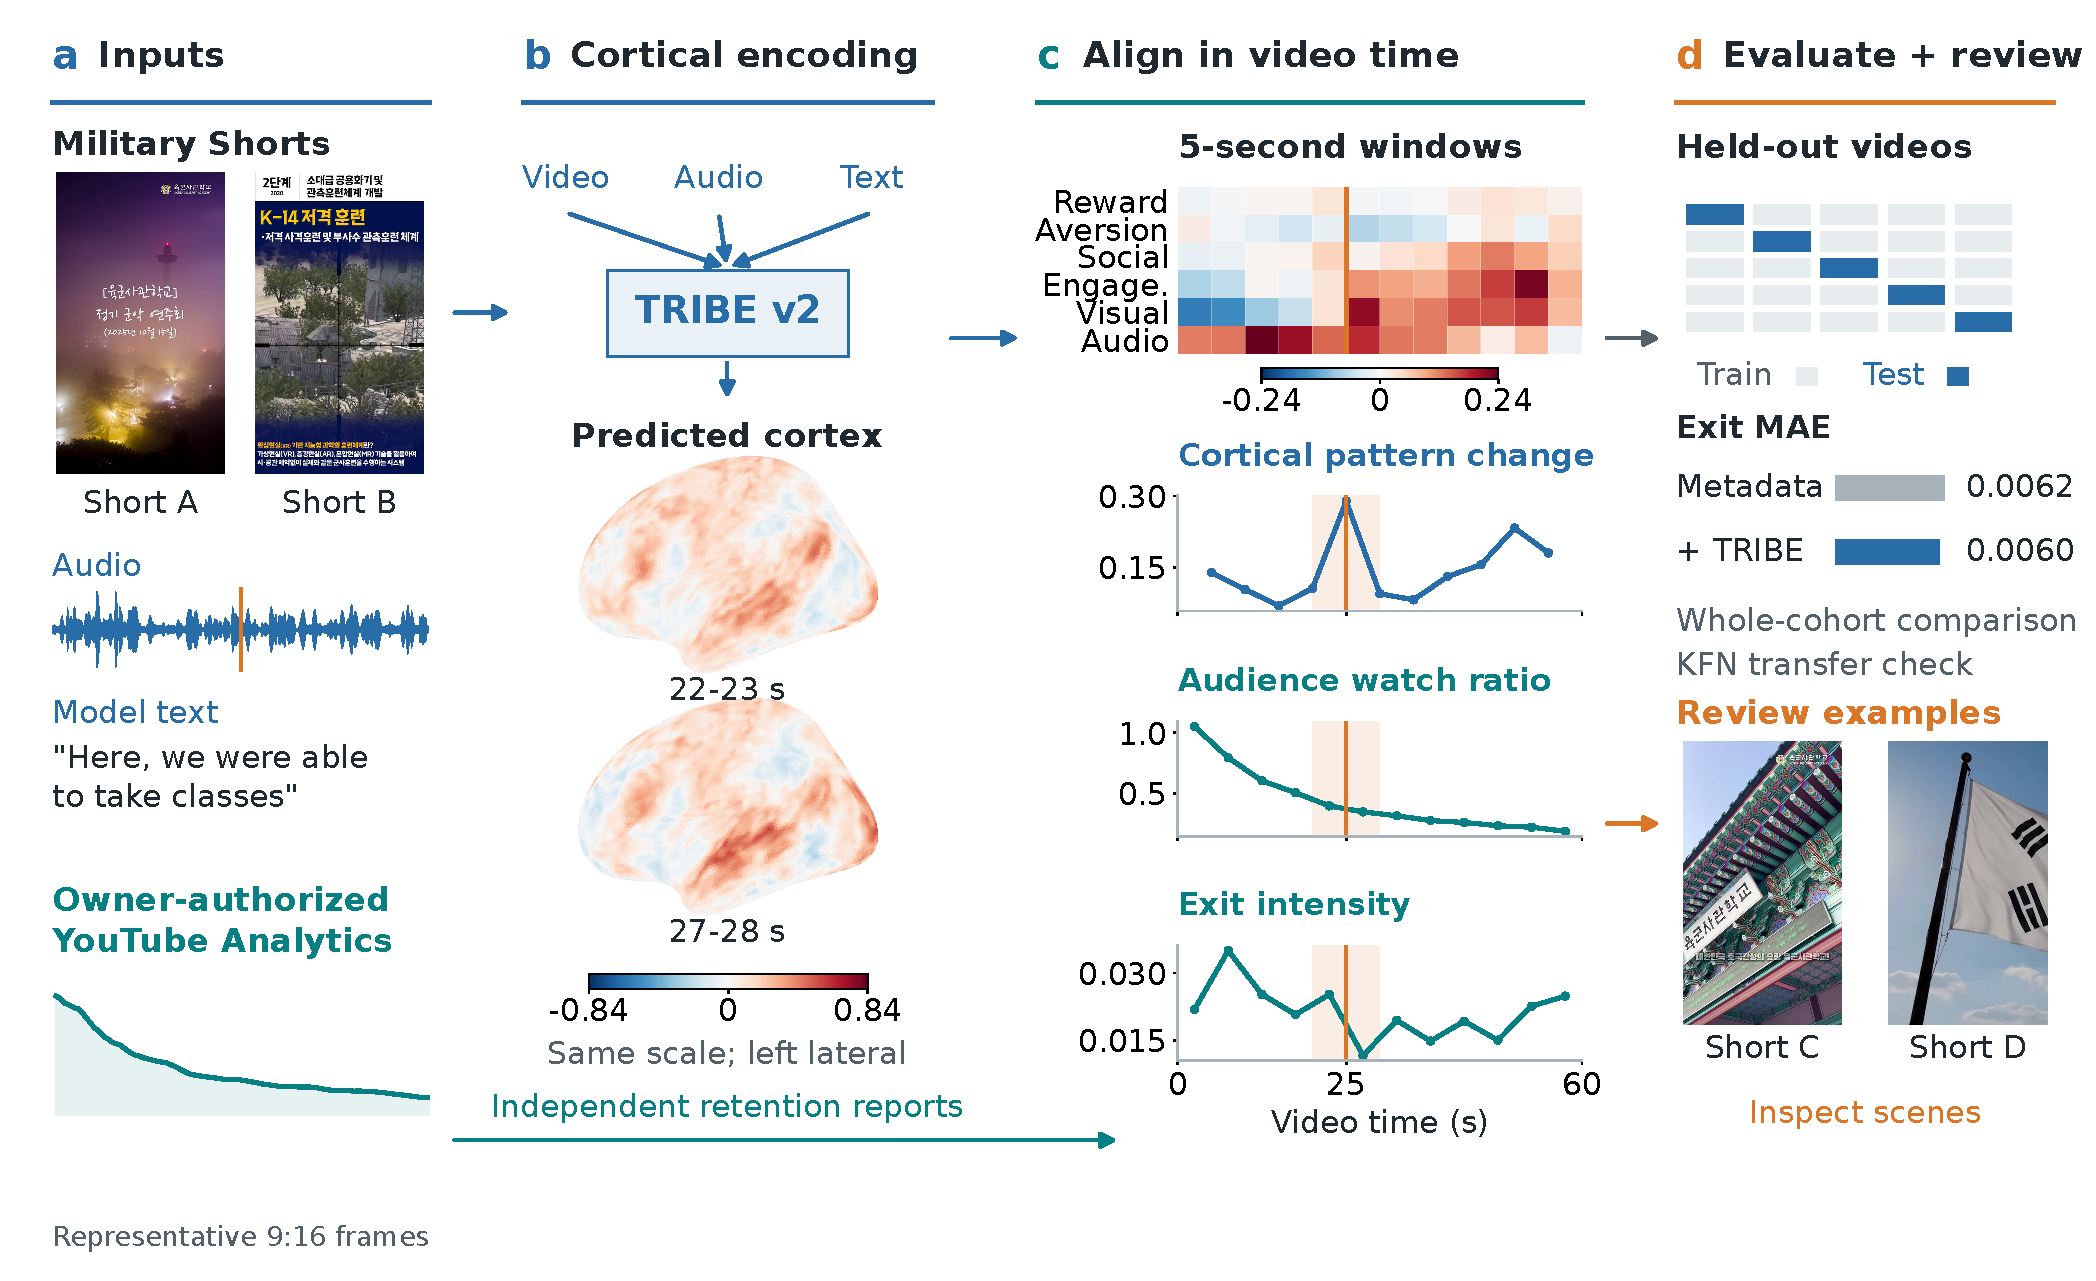
\includegraphics[width=\textwidth]{00_pipeline_overview.pdf}
\caption{Video-to-cortex workflow for time-aligned audience analysis and segment review.}
\label{fig:workflow}
\end{figure*}

\section{Related Work}
\label{sec:related}

\subsection{Audience behavior as an aggregate signal}
Audience-retention curves make an otherwise diffuse viewing process observable along a video-time axis, with platform-defined measures for elapsed position and audience behavior \cite{youtubeRetentionAPI}. Large-scale course and lecture-video studies show that engagement varies systematically with in-video position and that dropout and rewatching concentrate at identifiable timestamps \cite{breslow2013studying,kim2014dropouts}. Short-form platform research documents the reach and production culture of the format \cite{kaye2022tiktok} and its measurable interaction with long-form viewing \cite{rajendran2024shorts}. These curves can reveal broad position effects and local changes, but they remain aggregate platform statistics. They do not identify the reason for an individual departure, comprehension, or learning. This distinction is consistent with cautions in learning analytics that behavioral traces should be interpreted in relation to a substantive learning question rather than treated as self-sufficient evidence \cite{gasevic2015learning}. Here, retention is an external aggregate outcome for evaluating a content representation.

\subsection{Multimodal video representation}
Contemporary video understanding rests on learned multimodal and self-supervised representations: image--language contrastive models transfer natural-language supervision to vision \cite{radford2021clip}, multi-rate architectures capture temporal structure at coarse and fine resolutions \cite{feichtenhofer2019slowfast}, and latent-prediction models learn video representations without labels \cite{assran2025vjepa2}; survey treatments formalize how such synchronized streams are combined \cite{baltrusaitis2019multimodal}. The present representation retains synchronized visual, auditory, and language streams because TRIBE v2 is designed as a tri-modal model for naturalistic stimuli \cite{dascoli2026tribev2}. Evidence from online educational videos links production choices with observed viewing behavior \cite{guo2014video}; however, an aggregate viewing outcome does not by itself provide a time-local explanation of a particular channel's content. The present study retains the original multimodal model output and evaluates how it behaves when aligned with an independently collected platform report.

\subsection{Brain-predictive representations}
TRIBE v2 is a foundation model for predicting cortical responses to naturalistic audiovisual stimuli \cite{dascoli2026tribev2}, extending an earlier tri-modal whole-brain encoder \cite{dascoli2025tribe}. The underlying research program is well established: encoding models formally predict measured brain responses from stimulus features \cite{naselaris2011encoding}; natural-image identification \cite{kay2008identifying}, natural-movie reconstruction \cite{nishimoto2011naturalmovies}, and semantic maps derived from natural speech \cite{huth2016naturalspeech} related time-varying naturalistic stimuli to distributed cortical representations; and feature hierarchies optimized for vision proved predictive of cortical response patterns, including dynamic natural vision \cite{yamins2014performance,wen2018neural}. Parallel efforts align pretrained multimodal features to movie-evoked responses \cite{villanueva2025predicting}. Those studies motivate a structured stimulus representation; they do not validate the present channel application. A cortical-surface prediction is not equivalent to a measured response in a new audience. Its value here is narrower and testable: it supplies a structured, high-dimensional representation of stimulus content that can be summarized over time. An anatomical cortical atlas defines the parcel masks used for six region-based summaries; it provides spatial boundaries, not psychological labels or evidence that a viewer state occurred \cite{destrieux2010parcellation}.

\subsection{Prediction and explanation}
A model that improves a held-out error metric is not thereby a causal explanation of audience behavior. Prediction and explanation answer different questions and require different designs \cite{yarkoni2017prediction,shmueli2010explain}. Comparisons between matched training and test distributions further show that apparent generalization can disappear under distribution shift \cite{recht2019imagenet}. Accordingly, this paper reports error, robustness, and transfer behavior as evaluation results. It does not infer that a cortical descriptor causes retention, that a scene transition caused an audience change, or that the model can replace human editorial judgment.

\section{Data and Study Design}
\label{sec:data}

\subsection{Primary channel and frozen frame}
The primary frame was a frozen public Shorts-tab catalog for YugsaTV, an official military channel. The catalog contained 197 public items at the snapshot date. The channel owner authorized read-only access to YouTube Analytics for these reports. The analysis cutoff was September 12, 2026, and the Analytics reporting timezone was America/Los\_Angeles. Retention reports were queried from each video's publication date through the common cutoff; observation windows therefore differ across videos.

The unit of analysis is the video record and its time-indexed aggregate report. No participants were recruited or measured. The analysis contains no individual viewer records, individual service-member records, comment text, or private person-level data. Raw video and audio files are not redistributed. Owner-authorized Analytics responses remain private; only aggregate derived tables and figures needed for the manuscript are staged in the paper package.

\subsection{Nested inclusion frame}
The fixed inference run produced 194 strict, non-fallback TRIBE v2 outputs. Three catalog items were excluded before prediction because the run configuration rejected records whose unmatched-word ratio exceeded 0.05: \texttt{HnyZ72iYlH0} (1/18), \texttt{XiPeSUCdcHM} (1/1), and \texttt{nYGyDessKGY} (1/7). The threshold was fixed in the execution configuration before this result analysis; it was not preregistered. No audio-only, video-only, or simulated fallback was used. Among the 194 predicted videos, 190 returned non-empty retention reports. Four videos returned empty Analytics responses and were retained as missing rather than converted to zero retention. The primary five-second analysis contained 1,745 valid windows. Table~\ref{tab:coverage} reports the nested frame.

\begin{table*}[t]
\caption{Nested coverage of the primary owner-authorized analysis frame.}
\label{tab:coverage}
\centering
\scriptsize
\begin{tabularx}{\textwidth}{@{}lrlX@{}}
\toprule
Stage & Count & Role & Boundary \\
\midrule
Frozen public Shorts-tab catalog & 197 & Sampling frame & Dated channel snapshot, not all current or historical uploads. \\
Strict non-fallback TRIBE v2 outputs & 194 & Model-derived content representation & Predicted cortical values, not measured viewer neural activity. \\
Non-empty owner Analytics retention reports & 190 & Primary platform outcome & Aggregate reports, not individual viewing histories or learning outcomes. \\
Primary five-second windows & 1,745 & Within-video temporal unit & Windows from one video remain clustered within that video. \\
Six region-profile association screens & 140 & Video-level summaries & At least eight valid five-second observations per video after feature/outcome filtering. \\
Temporal-change association screens & 109 & Video-level summaries & Additional missing first-window or constant-vector values reduce the eligible video count. \\
KFN auxiliary strict outputs & 2,312 & Cross-channel stress test & Public-view analysis without owner-authorized retention curves. \\
\bottomrule
\end{tabularx}
\end{table*}

\subsection{Auxiliary channel}
KFN Shorts supplied a separate public-metadata stress test. Its frozen catalog contained 2,321 items and 2,312 strict, non-fallback outputs. Public view counts and model-derived summaries were used to test whether a representation calibrated on the primary channel transferred to a different channel. This is not a second owner-authorized retention study and is not evidence for a universal military-video law.

\section{Method}
\label{sec:method}

\subsection{Model-derived content representation}
TRIBE v2 processes synchronized visual, auditory, and language inputs \cite{dascoli2026tribev2} and produces predicted values on an fsaverage5 cortical surface with 20,484 vertices in the persisted run. In the persisted configuration, the visual stream uses frozen V-JEPA~2 features \cite{assran2025vjepa2}, the auditory stream uses a frozen W2v-BERT~2.0 checkpoint \cite{chung2021w2vbert}, and the language stream uses frozen Llama~3.2 features \cite{grattafiori2024llama3}; each backbone serves as a fixed feature extractor, consistent with the model's published configuration. The fsaverage5 surface is a standard coarse cortical reference geometry from the FreeSurfer suite \cite{fischl2012freesurfer}. Each video was presented to the model as a four-second, 64-frame clip. The persisted arrays in all 194 strict outputs contain contiguous one-second cortical intervals; the four-second input clip and one-second saved output interval are therefore distinct parts of the pipeline. The paper uses the persisted arrays and does not rerun the model during the audit.

The six region-based profiles are unweighted means of predicted cortical values over predefined parcel masks from an anatomical cortical atlas \cite{destrieux2010parcellation}. Their names are compact spatial labels: reward, aversion, social value, engagement, visual processing, and auditory processing. They are model-derived content features, not evidence that the named psychological or sensory state occurred in a viewer. Pattern change is calculated as one minus the correlation between adjacent cortical vectors after subtracting each vector's mean. In the primary windows, the vectors are adjacent overlap-weighted five-second aggregates of the persisted one-second outputs; the first comparison and constant-vector comparisons are undefined and omitted. This is a stimulus-representation change descriptor, not a neural event or physiological transition. The profile dictionary and parcel definitions are provided in Appendix A.

\subsection{Time alignment and outcomes}
The primary analysis used five-second windows; three- and ten-second windows were retained for sensitivity analysis. The one-second persisted cortical intervals and the Analytics one-percent position bins were mapped onto the same elapsed-video axis. Each analysis window was retained only when the cortical intervals covered it and the available Analytics bins covered it; cortical and Analytics values were combined with their respective temporal-overlap weights, and missing bins were not bridged. No additional hemodynamic or viewer-response delay was added.

Three primary outcomes were used. The first is the platform audience watch-ratio report, which can exceed one when repeat watching is included. The second is the platform's relative-retention report, interpreted according to its comparison definition. These platform definitions and the available elapsed-position fields are documented by YouTube \cite{youtubeRetentionAPI}. The third, exit intensity, was calculated for each aligned window as \(\texttt{stoppedWatching}/\texttt{totalSegmentImpressions}\). The two count fields were fractionally allocated from the one-percent Analytics bins by temporal overlap; if any required bin was missing, the window outcome was missing, and a zero or nonfinite denominator produced a missing value. Exit intensity is an aggregate segment statistic, not an individual hazard rate or a probability that a particular viewer exited. The exact platform field names are retained in the machine-readable audit tables.

\subsection{Position adjustment and association}
Retention can vary systematically with video position. In-video dropout studies report position-dependent audience behavior \cite{kim2014dropouts}, and multimedia-learning research treats segmentation of material as a first-order design factor \cite{mayer2009multimedia}. For each video, a cubic trend in normalized position was removed from both the feature and outcome series, following standard flexible-regression trend-removal practice \cite{hastie2009esl}. A within-video Spearman rank correlation was then computed on the residuals \cite{spearman1904association}. The reported estimate is the arithmetic mean of video-level correlations. Intervals use complete-video bootstrap resampling with 2,000 repetitions and seed 33, following the resampling logic introduced for the bootstrap method \cite{efron1979bootstrap}.

The submission audit applies the same cubic residualization before every circular-shift null correlation, in the spirit of surrogate-data testing for time series \cite{theiler1992surrogate}. It also constructs a matched transition for each high pattern-change event using the nearest non-event transition within the same video by normalized position. These checks are robustness diagnostics, not significance tests.

\subsection{Video-level prediction}
The primary prediction comparison uses video-grouped Ridge models \cite{hoerl1970ridge}. The metadata-only model contains duration, title length, description length, publication day, normalized position, and deterministic topic label. The two enriched feature sets add the six profile means and then the whole-cortex change descriptors. Standardization, imputation, categorical encoding, and Ridge alpha selection occur within the training fold; this separation matters because using the same data for model selection and error estimation can bias reported performance \cite{varma2006crossvalidation}. All windows from a video remain in one fold. A chronological 80/20 split provides a second time-ordered check. Mean absolute error (MAE) improvement is defined as metadata-only MAE minus enriched-model MAE, so positive values indicate lower error for the enriched model.

The audit also fits the same fixed HistGradientBoosting implementation from scikit-learn \cite{pedregosa2011scikit}, a histogram-based gradient boosting design in the LightGBM family \cite{ke2017lightgbm}, to metadata-only and enriched feature sets. This prevents an apparent nonlinear improvement from being attributed to TRIBE features when the algorithm has changed at the same time. These nonlinear results are reported in Appendix B; the interpretable Ridge comparison is the primary manuscript result.

\subsection{Pattern-change review candidates}
Within each video, candidate events were selected from the top decile of the pattern-change descriptor with at least ten seconds between candidates. A candidate required a contiguous preceding, current, and following five-second window, so endpoints and incomplete transitions were excluded. The adjacent before and after windows were compared. The matched control was the nearest non-event transition in the same video by normalized position. The procedure produced 93 candidate transitions across 85 videos and 92 complete event-control pairs across 84 videos; the mean normalized-position distance was 0.1918. The resulting display is a review queue: it identifies locations for a human to inspect, not scenes that an algorithm should automatically remove.

\subsection{Reproducibility and data governance}
The analysis was run from the immutable aggregate-analysis manifest and the verified local TRIBE release. The submission audit records the source hashes, the 0.05 alignment threshold, four-second model input clip, one-second persisted interval, three/five/ten-second window widths, analysis cutoff, timezone, seed, bootstrap count, null permutations, feature sets, and fold rules. The repository contains code, aggregate tables, figure files, and checksums, following the findable, accessible, interoperable, and reusable data-stewardship principles for the aggregate artifacts \cite{wilkinson2016fair}. Raw media, model weights, runtime caches, raw Analytics responses, and private owner records are excluded. The final data-access statement must be replaced with the author-approved route and must reflect YouTube, model, and institutional constraints.

\section{Results}
\label{sec:results}

\subsection{Retention structure and position effect}
The primary frame retained 194 strict model outputs and 190 videos with non-empty owner-authorized retention reports. Figure~\ref{fig:retention} shows the median and 10th--90th percentile envelope of audience watch ratio over normalized video position. The broad position pattern motivates residualization before feature comparison. The envelope is descriptive; it is not a survival curve and does not identify a causal point of audience departure.

\begin{figure*}[t]
\centering
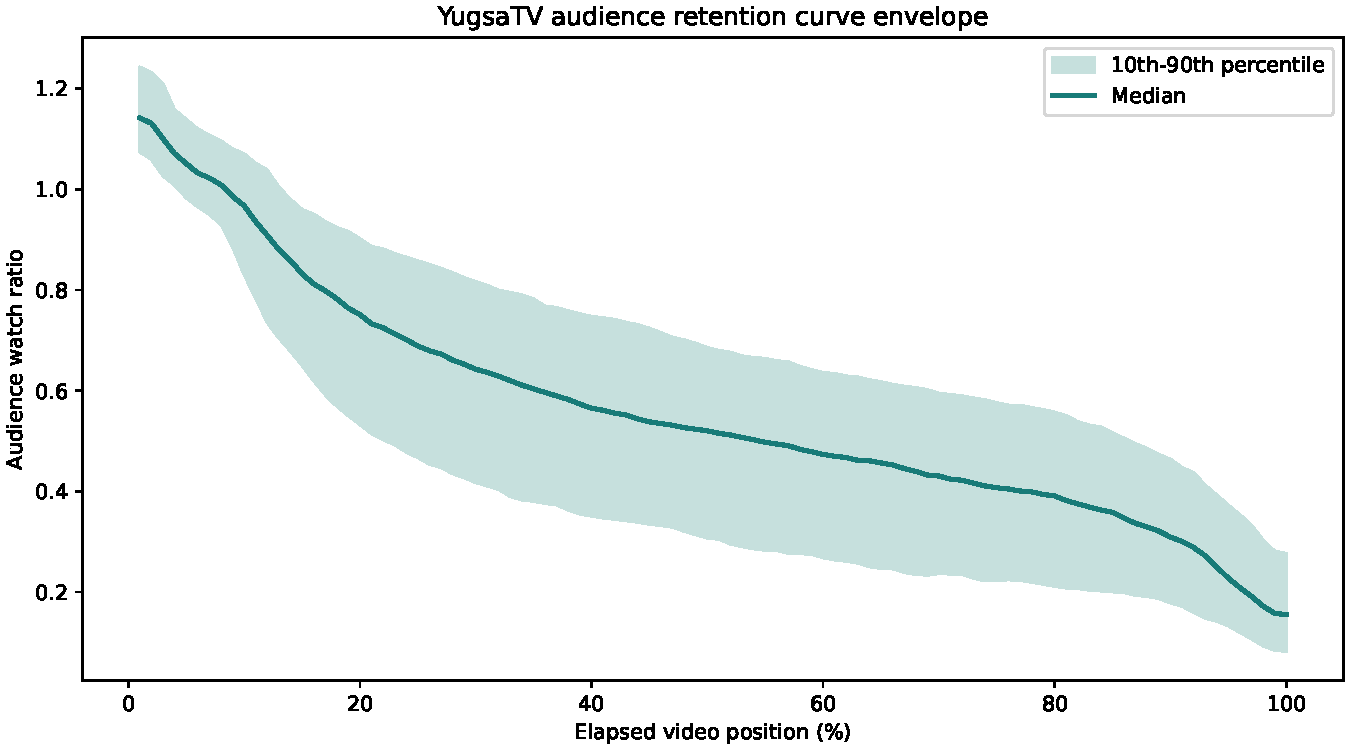
\includegraphics[width=0.95\textwidth]{04_retention_curve_envelope.pdf}
\caption{Aggregate audience-watch-ratio envelope across normalized video position.}
\label{fig:retention}
\end{figure*}

\subsection{What the cortical representation contains}
Figure~\ref{fig:cortical} projects the duration-weighted, video-level whole-cortex predictions into their first two principal components, a descriptive dimensionality-reduction view \cite{jolliffe2016pca}. The first two components explain 75.4\% of the variance in the current 194-video representation. The plot is a descriptive map of model-derived content patterns; its view-count color scale is contextual and does not establish a view-count mechanism or a viewer group separation. It shows why the analysis retains both region summaries and time-local changes rather than reducing the representation to one composite score.

\begin{figure*}[t]
\centering
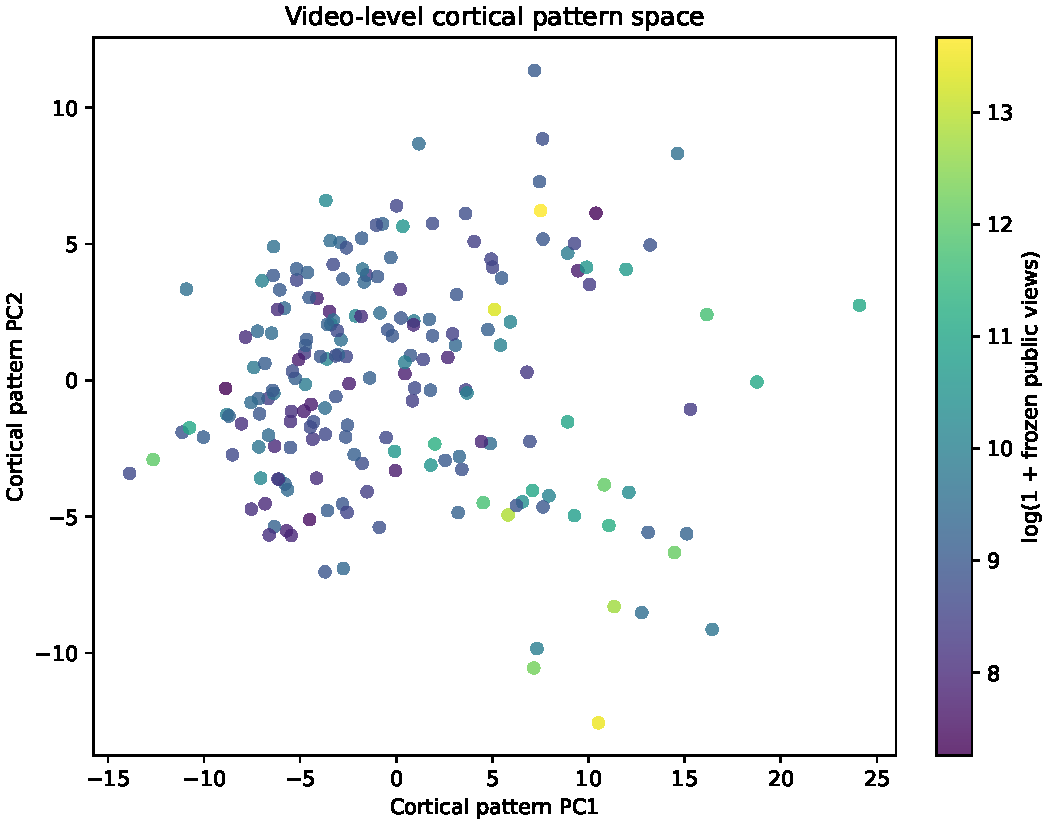
\includegraphics[width=0.82\textwidth]{07_cortical_pca.pdf}
\caption{Descriptive principal-component view of video-level cortical pattern representations.}
\label{fig:cortical}
\end{figure*}

\subsection{Position-adjusted associations}
Figure~\ref{fig:associations} and Table~\ref{tab:associations} summarize the primary associations. Social value had the largest mean association with audience watch ratio ($\rho=0.437$, 95\% video-bootstrap interval $[0.361,0.508]$, 140 videos), followed by aversion ($\rho=0.417$, $[0.339,0.490]$). Pattern change had the largest association with exit intensity ($\rho=0.281$, $[0.195,0.366]$, 109 videos). The same feature pattern was weaker for relative retention performance, where social value reached $\rho=0.347$.

The position-adjusted circular-shift audit produced near-zero null means for the same comparisons: social value and aversion were approximately $-0.011$ and $-0.009$ for audience watch ratio, while pattern change was approximately $-0.026$ for exit intensity. These values are included as a design check rather than converted into a claim of statistical significance.

\begin{figure*}[t]
\centering
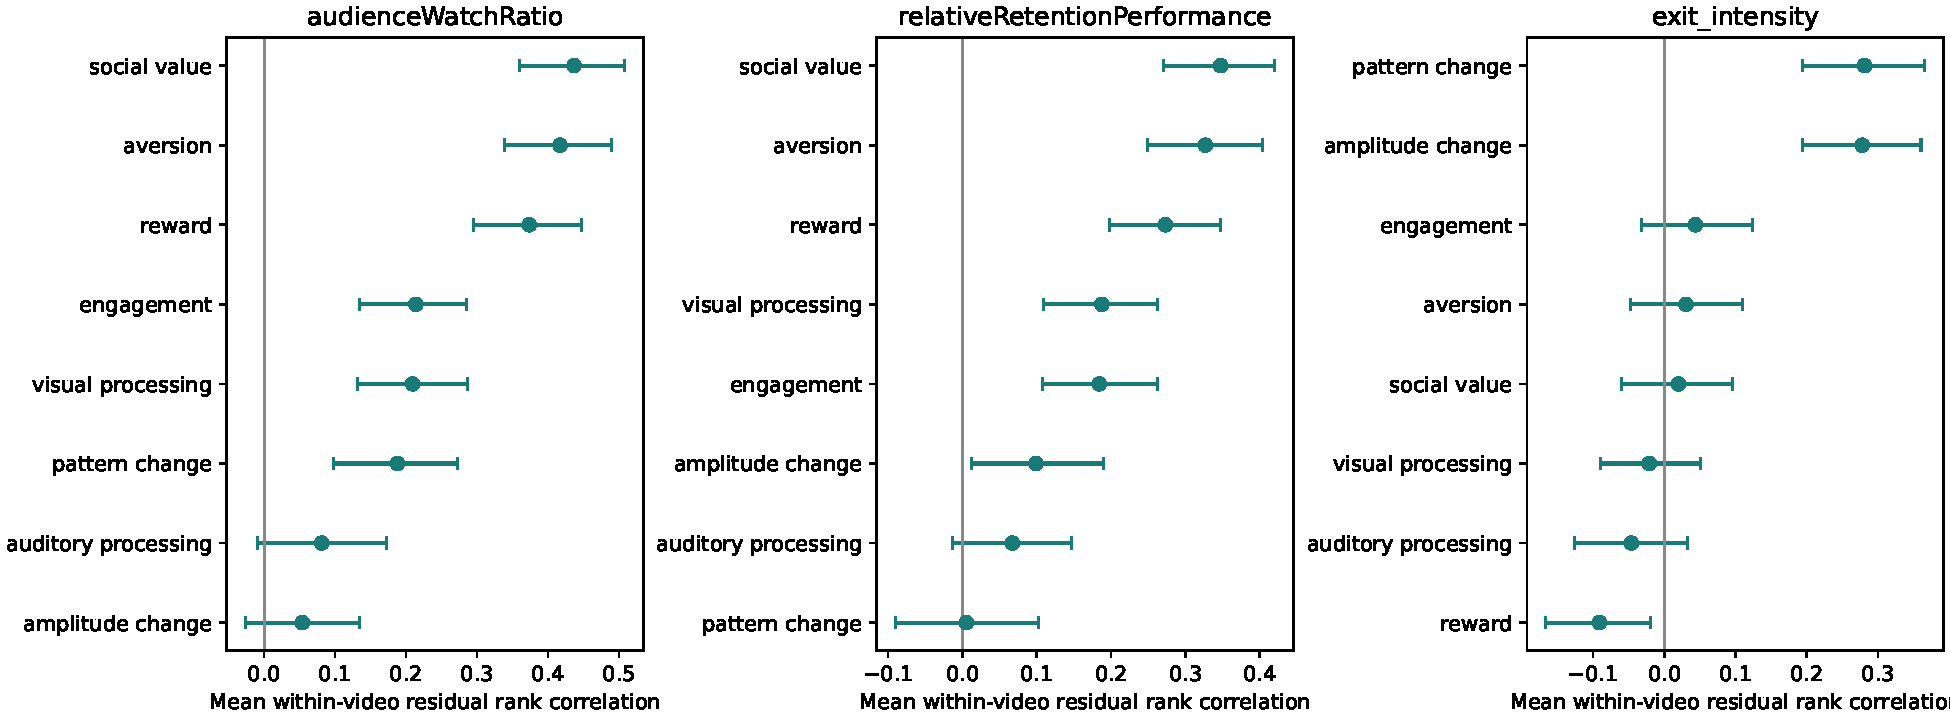
\includegraphics[width=0.98\textwidth]{01_continuous_associations.pdf}
\caption{Position-adjusted within-video associations between model-derived content features and platform outcomes.}
\label{fig:associations}
\end{figure*}

\begin{table*}[t]
\caption{Selected position-adjusted associations in the primary frame.}
\label{tab:associations}
\centering
\scriptsize
\begin{tabular}{@{}lllll@{}}
\toprule
Outcome & Feature & Videos & Mean $\rho$ & 95\% video-bootstrap interval \\
\midrule
Audience watch ratio & Social value & 140 & 0.437 & [0.361, 0.508] \\
Audience watch ratio & Aversion & 140 & 0.417 & [0.339, 0.490] \\
Audience watch ratio & Reward & 140 & 0.374 & [0.295, 0.447] \\
Relative retention performance & Social value & 140 & 0.347 & [0.270, 0.420] \\
Exit intensity & Pattern change & 109 & 0.281 & [0.195, 0.366] \\
Exit intensity & Amplitude change & 109 & 0.278 & [0.194, 0.360] \\
\bottomrule
\end{tabular}
\end{table*}

\subsection{Incremental prediction is outcome-specific}
The same-family Ridge comparison is shown in Figure~\ref{fig:prediction} and Table~\ref{tab:prediction}. Adding region means and temporal changes reduced grouped exit-intensity MAE from 0.006237 to 0.005954, a video-equal improvement of 0.000283 with a 95\% bootstrap interval of [0.000124, 0.000442]. The chronological point estimate changed from 0.006476 to 0.006090, but its interval included zero (improvement 0.000386, 95\% interval [-0.000013, 0.000791]). In contrast, grouped audience-watch-ratio MAE changed from 0.092979 to 0.094006, and relative-retention MAE changed from 0.076750 to 0.076372. The result supports an outcome-specific additional-information claim, not a universal improvement claim.

\begin{figure*}[t]
\centering
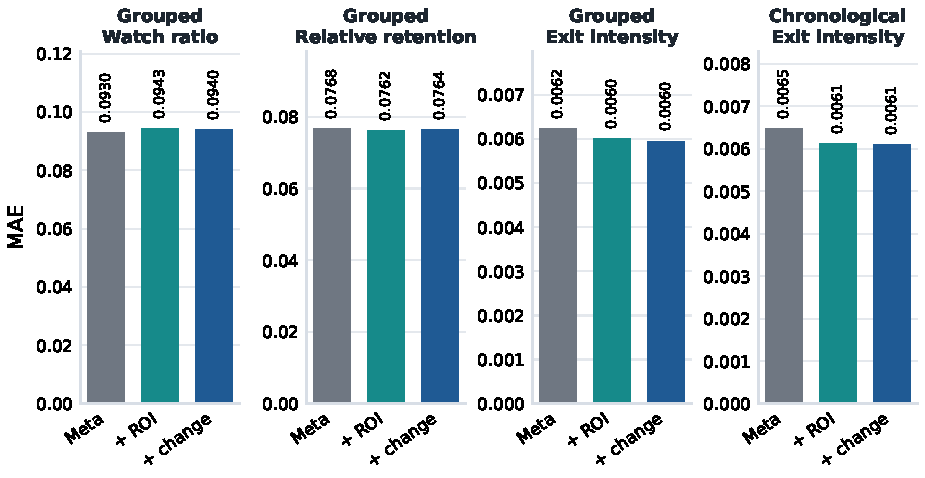
\includegraphics[width=0.98\textwidth]{02_predictive_increment.pdf}
\caption{Same-family Ridge error comparison for metadata, region profiles, and temporal changes; bars are video-equal MAE for grouped evaluation or the chronological check.}
\label{fig:prediction}
\end{figure*}

\begin{table*}[t]
\caption{Fair video-level Ridge comparison for primary outcomes.}
\label{tab:prediction}
\centering
\scriptsize
\begin{tabular}{@{}lllrrrr@{}}
\toprule
Outcome & Split & Feature set & Videos & MAE & $R^2$ & Pooled Spearman \\
\midrule
Audience watch ratio & Grouped & Metadata & 190 & 0.092979 & 0.784 & 0.843 \\
Audience watch ratio & Grouped & Metadata + ROI & 190 & 0.094338 & 0.781 & 0.849 \\
Audience watch ratio & Grouped & Metadata + ROI + changes & 190 & 0.094006 & 0.780 & 0.849 \\
Relative retention & Grouped & Metadata & 190 & 0.076750 & 0.375 & 0.623 \\
Relative retention & Grouped & Metadata + ROI & 190 & 0.076229 & 0.374 & 0.622 \\
Relative retention & Grouped & Metadata + ROI + changes & 190 & 0.076372 & 0.371 & 0.620 \\
Exit intensity & Grouped & Metadata & 190 & 0.006237 & 0.470 & 0.627 \\
Exit intensity & Grouped & Metadata + ROI & 190 & 0.006017 & 0.522 & 0.617 \\
Exit intensity & Grouped & Metadata + ROI + changes & 190 & 0.005954 & 0.536 & 0.616 \\
Exit intensity & Chronological & Metadata & 38 & 0.006476 & 0.302 & 0.602 \\
Exit intensity & Chronological & Metadata + ROI & 38 & 0.006127 & 0.353 & 0.619 \\
Exit intensity & Chronological & Metadata + ROI + changes & 38 & 0.006090 & 0.358 & 0.598 \\
\bottomrule
\end{tabular}
\end{table*}

\subsection{Pattern-change locations form a review queue}
The event analysis identified 93 candidate transitions across 85 videos; 92 matched event/control pairs across 84 videos had complete values for the primary display. At event transitions, audience watch ratio changed by -0.150 compared with -0.069 at the matched control transitions. Exit intensity changed by +0.00505 at events compared with -0.00207 at controls. The corresponding descriptive event-minus-control contrasts were -0.0811 and +0.00713, respectively. Relative retention changed by -0.0215 at events compared with +0.0279 at controls, for a contrast of -0.0493. Figure~\ref{fig:events} presents the three outcome-specific contrasts. The result identifies locations worth editorial inspection; it does not show that a cortical-pattern change caused an audience change.

\begin{figure*}[t]
\centering
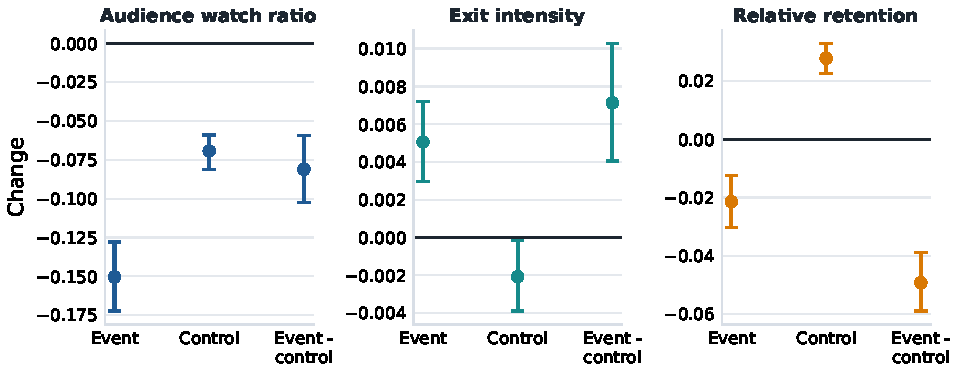
\includegraphics[width=0.95\textwidth]{05_pattern_change_events.pdf}
\caption{Matched outcome contrasts around high whole-cortex pattern-change locations; 92 pairs from 84 videos, with five-second overlap-weighted windows and 95\% video-bootstrap intervals.}
\label{fig:events}
\end{figure*}

\subsection{Cross-channel transfer is not established}
The auxiliary public-view stress test did not support direct cross-channel generalization. A model trained on YugsaTV and evaluated on KFN produced held-out $R^2$ values of -0.306 and -0.183 for metadata-only and metadata-plus-profile models, respectively. Training on KFN and evaluating on YugsaTV produced -0.755 and -1.348. These negative values indicate performance below the test-set mean baseline, not negative correlations. Figure~\ref{fig:transfer} therefore functions as a boundary result: the primary-channel relationships should not be treated as a universal law for military video.

\begin{figure*}[!t]
\centering
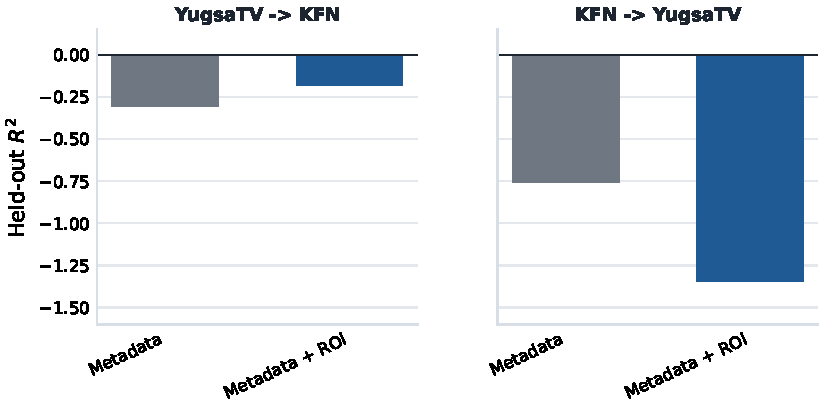
\includegraphics[width=0.82\textwidth]{03_cross_channel.pdf}
\caption{Auxiliary cross-channel held-out transfer using public view counts; training/testing video counts are 194/2,312 and 2,312/194, respectively.}
\label{fig:transfer}
\end{figure*}

\section{Discussion}
\label{sec:discussion}

The results answer the three research questions with different strengths. First, after removing the common position trend, several model-derived profiles were associated with aggregate retention summaries, and whole-cortex pattern change was associated with exit intensity. The profiles represent model-derived content features rather than viewer psychological states; their associations with platform outcomes do not show that the named processes occurred. Second, adding the profiles and temporal changes reduced exit-intensity error in the grouped Ridge evaluation, while the chronological point estimate was smaller but uncertain under its bootstrap interval. The addition did not improve every outcome. Third, the event procedure creates a concrete review queue containing a location, a model-derived change, an aggregate outcome contrast, and a question for a human reviewer.

The workflow has two distinct uses. Before publication, TRIBE-derived content descriptors can nominate high-change or high-error segments for human review from the candidate video itself; observed retention and prediction error are not yet available. After publication, the same descriptors can be aligned with observed aggregate platform outcomes to identify segments where content changes and audience behavior warrant joint inspection. This preserves which profile, which time interval, and which outcome contributed to the review cue rather than collapsing them into a composite score; composite-indicator methodology makes the same point analytically, since aggregation choices can hide the drivers of an index \cite{nardo2005composite}. The workflow does not automatically prescribe an edit, certify educational quality, or evaluate an individual service member.

The negative transfer result clarifies the scope of the contribution. A representation that is useful for one channel's temporal review need not be calibrated for another channel, paralleling reports that models fitted on one distribution can fail on nominally matched test data \cite{recht2019imagenet}. In the present study, the two channel analyses differ in channel context and available platform outcomes; because those factors were not experimentally controlled, the transfer result cannot identify which unmeasured factor explains the difference. The next study should therefore freeze the analysis procedure before observing a new upload cohort and evaluate prospective generalization rather than repeatedly searching a completed cohort.

Several limitations remain. The primary Analytics period differs by upload date, and four videos had empty retention responses. The six profiles are spatial summaries of model predictions and should not be read as measurements of viewer brain activity or psychological states. Retention is an aggregate platform outcome and cannot establish comprehension, learning, or the reason for an individual departure. The feature screens were not preregistered, and the current work is a retrospective exploratory evaluation; preregistration exists precisely to separate such exploratory analysis from confirmatory claims \cite{nosek2018preregistration}. Even with position matching, a selected pattern-change event may coincide with a scene boundary or an unmeasured production change. Finally, the auxiliary KFN analysis uses public counts rather than owner-authorized retention reports and is therefore a transfer stress test, not an independent validation cohort.

The most informative next test is prospective. Before new uploads, fix the primary outcome, feature groups, fold rule, window rule, null procedure, and reporting table. After publication, use only the frozen procedure to nominate review segments, then ask trained human reviewers whether the nominations correspond to actionable content issues. A controlled editing study would be required to establish whether this review process changes production decisions or improves educational outcomes; such questions belong to the experimental and quasi-experimental design tradition rather than to observational association screens \cite{shadish2002experimental}.

\section{Conclusion}
\label{sec:conclusion}

This study established an auditable procedure for joining temporal TRIBE v2 content representations with owner-authorized YouTube audience-retention reports. In the primary YugsaTV frame, social-value and aversion profiles showed the largest position-adjusted associations with audience watch ratio, while pattern change was associated with segment-level exit intensity. Adding cortical profiles and temporal changes provided outcome-specific additional information for exploratory exit-intensity evaluation, while cross-channel transfer was not established. The procedure can support human review of time-local editorial candidates before publication and structured comparison with observed platform outcomes after publication. Its findings do not establish editing or educational effects, and the model-derived profiles are not measurements of viewer brains, psychological states, learning, or military readiness.

\clearpage
\appendices

\section{Feature and Outcome Definitions}
\label{app:definitions}

Table~\ref{tab:profiles} defines the six region-based profiles used in the manuscript. Each profile is an unweighted mean of predicted cortical values over the listed parcel masks from the anatomical cortical parcellation used for spatial aggregation \cite{destrieux2010parcellation}. The labels are spatial shorthand for reproducible aggregation and are not claims about a viewer's psychological state.

\begin{table*}[!b]
\caption{Region-based content profiles used in the primary analysis.}
\label{tab:profiles}
\centering
\scriptsize
\begin{tabularx}{\textwidth}{@{}lllX@{}}
\toprule
Profile & Parcel summary & Output role & Interpretation boundary \\
\midrule
Reward & Frontomarginal and rectus gyri & Region-based cortical content descriptor & Does not establish reward or positive affect in a viewer. \\
Aversion & Short insular gyrus and anterior circular insular sulcus & Region-based cortical content descriptor & Does not establish avoidance, discomfort, or rejection. \\
Social value & Anterior-mid cingulate and angular parietal parcels & Region-based cortical content descriptor & Does not establish social valuation or a social judgment. \\
Engagement & Dorsal and ventral posterior cingulate parcels & Region-based cortical content descriptor & Does not establish attention, immersion, or viewing persistence. \\
Visual processing & Calcarine, cuneus, and medial occipito-temporal parcels & Region-based cortical content descriptor & Describes a model summary of visual stimulus content. \\
Auditory processing & Planum temporale and transverse temporal parcels & Region-based cortical content descriptor & Describes a model summary of auditory stimulus content. \\
\bottomrule
\end{tabularx}
\end{table*}
The whole-cortex pattern-change descriptor is one minus the correlation between adjacent cortical vectors after within-vector centering. The persisted TRIBE outputs are one-second intervals; for the primary analysis, these are overlap-weighted into adjacent five-second windows before the pattern-change calculation. The first comparison and any constant-vector comparison are undefined and omitted. No composite score is formed by summing the six profiles.

% Flush Appendix A's wide table before beginning the audit appendix.
\clearpage
\section{Submission Audit and Robustness Results}
\label{app:audit}

The submission audit was run from the frozen extended-analysis tables without media collection, model loading, OAuth access, or GPU inference. The audit output is identified by the \texttt{audit\_manifest.json} file in the submission-audit directory. The inference configuration used a four-second, 64-frame model input clip and produced one-second persisted cortical intervals. The analysis used five-second windows with temporal-overlap weighting, seed 33, 500 circular shifts per video-feature-outcome combination, and the fold rules recorded in the manifest. The text-event alignment exclusion threshold was 0.05 unmatched words divided by word records; it was an execution setting, not a preregistered decision.

The main position-adjusted comparisons were recomputed after applying the same cubic residualization to observed and shifted feature series. Table~\ref{tab:null} reports the key observed and null means. The null values are design diagnostics; they are not reported as a new multiple-testing significance procedure.

\begin{table*}[!b]
\caption{Position-adjusted circular-shift audit for selected associations.}
\label{tab:null}
\centering
\scriptsize
\begin{tabular}{@{}llrrrr@{}}
\toprule
Outcome & Feature & Videos & Observed mean $\rho$ & Null mean $\rho$ & Observed minus null \\
\midrule
Audience watch ratio & Social value & 140 & 0.437 & -0.011 & 0.448 \\
Audience watch ratio & Aversion & 140 & 0.417 & -0.009 & 0.426 \\
Audience watch ratio & Reward & 140 & 0.374 & -0.018 & 0.392 \\
Exit intensity & Pattern change & 109 & 0.281 & -0.026 & 0.307 \\
Exit intensity & Amplitude change & 109 & 0.278 & -0.016 & 0.293 \\
\bottomrule
\end{tabular}
\end{table*}

For the matched event control, 92 transition pairs were available across 84 videos. The event-minus-control arithmetic contrasts were -0.0811 for audience watch ratio, +0.00713 for exit intensity, and -0.0493 for relative retention performance. The mean normalized-position distance between event and control transitions was 0.192. These values support retaining the event display as a review-candidate analysis while keeping its interpretation descriptive; they are not causal difference-in-differences estimates \cite{bertrand2004did}.

The fair model audit compared three feature sets under both Ridge and the same fixed HistGradientBoosting model, a histogram-based gradient boosting design in the LightGBM family \cite{ke2017lightgbm}: metadata only, metadata plus six profiles, and metadata plus profiles plus temporal changes. All preprocessing and Ridge alpha selection occurred inside the training fold, and video identity was kept intact across folds. Keeping model selection inside the training fold avoids the error-estimation bias described for cross-validation model selection \cite{varma2006crossvalidation}. Table~\ref{tab:nonlinear} gives the nonlinear exit-intensity comparison; the primary manuscript uses Ridge because its feature-set comparison is easier to audit and explain.

\begin{table*}[!b]
\caption{Same-family nonlinear audit for exit intensity.}
\label{tab:nonlinear}
\centering
\scriptsize
\begin{tabular}{@{}lllrrr@{}}
\toprule
Split & Feature set & Videos & MAE & $R^2$ & Pooled Spearman \\
\midrule
Grouped & Metadata & 190 & 0.005394 & 0.580 & 0.643 \\
Grouped & Metadata + profiles + changes & 190 & 0.005309 & 0.605 & 0.638 \\
Chronological & Metadata & 38 & 0.006209 & 0.395 & 0.629 \\
Chronological & Metadata + profiles + changes & 38 & 0.006014 & 0.420 & 0.611 \\
\bottomrule
\end{tabular}
\end{table*}

The stored window-sensitivity analysis changes the width used to form the
within-video high-versus-low outcome contrast while retaining the common
140-video cohort. Table~\ref{tab:sensitivity} reports the contrast for the
three profiles that are most visible in the primary audience-watch-ratio
association display. Each value is the profile mean in the top-quartile
audience-watch-ratio windows minus the profile mean in the bottom-quartile
windows, computed within each video and then summarized across videos. A
negative value therefore means that the model-derived profile value was lower
in the high-watch windows under this descriptive comparison; it does not
indicate a causal effect or a viewer state. Their purpose is to show how the
profile ordering behaves when the temporal aggregation changes from three to
ten seconds.

\begin{table*}[!b]
\caption{Window-width sensitivity for selected audience-watch-ratio contrasts.}
\label{tab:sensitivity}
\centering
\scriptsize
\begin{tabular}{@{}llrrr@{}}
\toprule
Feature & Window width (s) & Videos & High-watch minus low-watch profile mean & 95\% video-bootstrap interval \\
\midrule
Social value & 3  & 140 & -0.128 & [-0.136, -0.119] \\
Social value & 5  & 140 & -0.111 & [-0.120, -0.103] \\
Social value & 10 & 140 & -0.086 & [-0.093, -0.078] \\
Aversion & 3  & 140 & -0.105 & [-0.114, -0.098] \\
Aversion & 5  & 140 & -0.089 & [-0.097, -0.081] \\
Aversion & 10 & 140 & -0.063 & [-0.070, -0.056] \\
Reward & 3  & 140 & -0.031 & [-0.034, -0.029] \\
Reward & 5  & 140 & -0.029 & [-0.031, -0.026] \\
Reward & 10 & 140 & -0.023 & [-0.025, -0.020] \\
\bottomrule
\end{tabular}
\end{table*}

\section{Extended Descriptive Analyses}
\label{app:extended}

The following analyses were completed from the same frozen result set and are retained for transparency rather than promoted to primary claims. Topic summaries describe distributions of content labels and outcomes. Retention-cluster candidates describe curve shape and are not validated audience types. The full three-, five-, and ten-second window sensitivity tables, all cortical parcel screens, API-context associations, and video-level out-of-fold predictions remain in the aggregate audit and extended-analysis directories.

\begin{figure*}[!t]
\centering
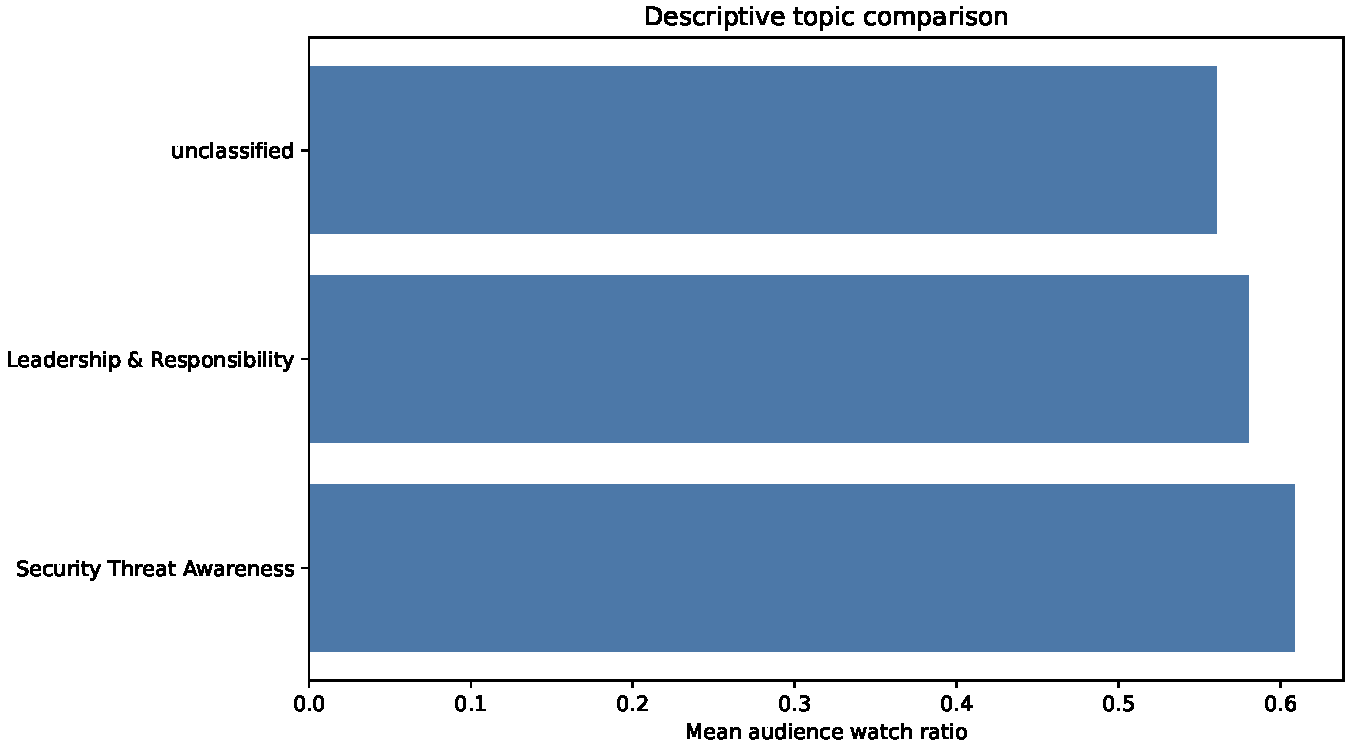
\includegraphics[width=0.47\textwidth]{06_topic_summary.pdf}\hfill
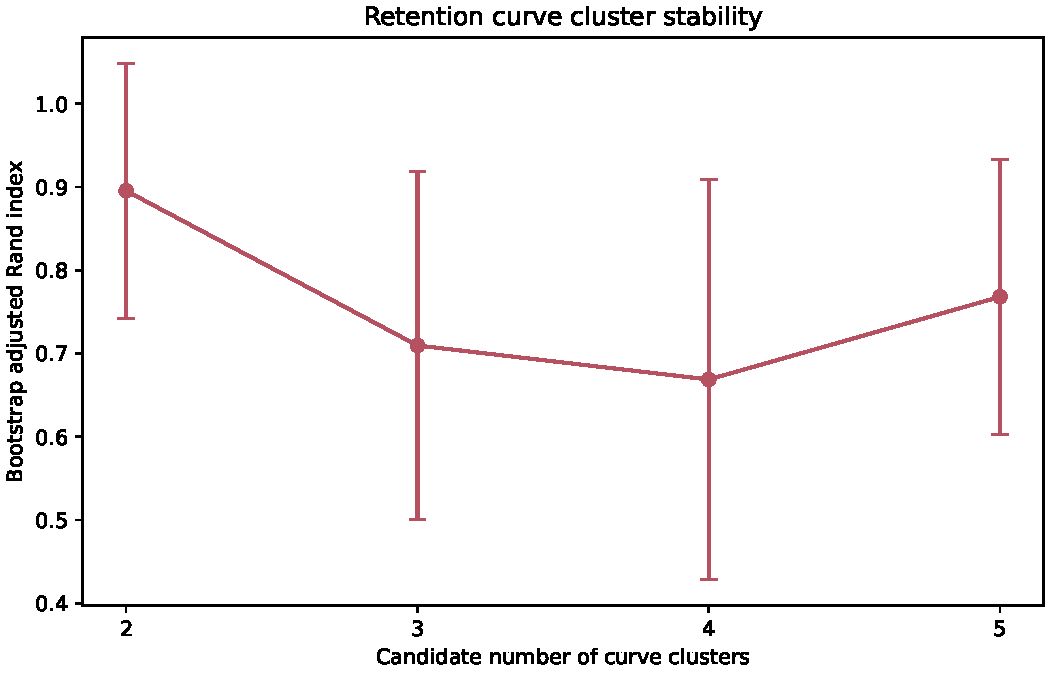
\includegraphics[width=0.47\textwidth]{08_retention_cluster_stability.pdf}
\caption{Extended descriptive analyses: (a) retention summaries across deterministic content labels and (b) stability checks for candidate retention-curve cluster counts.}
\label{fig:extended}
\end{figure*}

\section{Reproducibility Record}
\label{app:repro}

The primary analysis used four-second, 64-frame model input clips, one-second persisted cortical intervals, five-second analysis windows, bootstrap seed 33, 2,000 video-bootstrap repetitions, grouped five-fold evaluation, a chronological 80/20 check, and a Ridge alpha grid of $[0.01,0.1,1,10,100,1000]$. The submission audit added 500 position-adjusted circular shifts per eligible combination and a matched-position event control. Source and derived-file hashes are recorded in the original extended-analysis \texttt{MANIFEST.json}, the submission-audit \texttt{audit\_manifest.json}, and the paper-package figure provenance. The public package excludes raw media, private Analytics responses, credentials, model weights, and runtime caches.


% Flush all appendix tables and figures before the declarations and references.
% Keep the short declaration blocks compact instead of stretching inter-section
% glue to fill the page.
\clearpage
\begingroup
\raggedbottom

\section*{Data Availability}
Code, sanitized public metadata, derived aggregate analysis tables, figure files, configuration records, and checksums will be deposited in a public, versioned research repository with a persistent DOI upon publication. Raw video and audio, raw YouTube Analytics responses, model weights, runtime caches, and other private owner-authorized records are not redistributed. The repository DOI and access link will be added to this statement before submission.

\section*{Ethics and Governance}
No human participants were recruited, assigned, or measured. The analysis used public video records and owner-authorized aggregate channel reports; therefore, institutional research-ethics review was not required.

% Keep the acknowledgment paragraph intact in the next column.
\newpage
\section*{Acknowledgment}
This work was supported by the 2026 research fund of the Korea Military Academy (Hwarangdae Research Institute).

This draft was prepared with assistance from generative artificial intelligence tools for language drafting, code and document inspection, and LaTeX package preparation \cite{openAICodex}. The authors must review, verify, and take responsibility for all text, numerical results, citations, declarations, and interpretations before submission. The final manuscript must follow the IEEE policy for identifying sections that used AI-generated text and citing the AI system used.

% Keep the reference list out of the declaration-page flow.
\clearpage
\endgroup
\bibliographystyle{IEEEtran}
\bibliography{references}

\begin{IEEEbiographynophoto}{AUTHOR NAME}
AUTHOR NAME biography is pending author approval. Replace this placeholder with a concise biography covering the author's affiliation, relevant education or experience, and research interests.
\end{IEEEbiographynophoto}

\EOD
\end{document}
